% A common loop-topological carrier for electroweak and emergent-gravity sectors
% Bridge Note companion to Papers 1-4 of the Emergence reproducibility-paper series

\documentclass[11pt,a4paper]{article}

\usepackage{amsmath,amssymb,amsthm}
\usepackage{graphicx}
\PassOptionsToPackage{hyphens}{url}
\usepackage[colorlinks=true,linkcolor=blue,citecolor=blue,urlcolor=blue,breaklinks=true]{hyperref}
\hypersetup{
  pdftitle={A common loop-topological carrier for electroweak and emergent-gravity sectors},
  pdfauthor={Sandro Bucciarelli},
  pdfsubject={Relational carrier theory},
}
\makeatletter
\g@addto@macro\UrlBreaks{\do\_\do\/\do\.\do\-}
\makeatother
\usepackage[margin=2.5cm]{geometry}
\usepackage{booktabs}
\usepackage{xcolor}
\usepackage{cite}

% Clickable GitHub links for src/*.py citations (auto-generated)
\newcommand{\ghrepo}[1]{https://github.com/TerraSignum/#1}
% \nolinkurl gives a monospace, line-breakable rendering (handles
% underscores) without creating an inner link competing with \href.
\newcommand{\pyscript}[3]{%
  \href{\ghrepo{#1}/blob/main/#2}{\nolinkurl{#3}}}
\newcommand{\repoOwn}{qft-einstein-bridge-repro}
\newcommand{\pyown}[2]{\pyscript{\repoOwn}{#1}{#2}}

\title{A common loop-topological carrier for electroweak\\
       and emergent-gravity sectors\\
       \large (Technical consistency note across Papers~1--4)}
\author{Sandro Bucciarelli\thanks{Independent researcher.
        Correspondence: \href{mailto:sandro.bucciarelli89@gmail.com}{sandro.bucciarelli89@gmail.com}.}}
\date{\today}

\newcommand{\esync}{\varepsilon_{\mathrm{sync}}^{2}}
\newcommand{\axi}{\alpha_{\xi}}
\newcommand{\DOmega}{D(\Omega)}
\newcommand{\bpi}{\beta_{\pi}}
\newcommand{\Lib}{\mathcal{L}}
\newcommand{\msbar}{\overline{\mathrm{MS}}}

\emergencystretch=5em
\hbadness=10000
\hfuzz=2pt
\sloppy

\begin{document}
\maketitle

\begin{abstract}
\noindent\textbf{This note performs a cross-file consistency
audit across the four companion papers of the corpus
(Papers~1--4).} It is a \emph{technical consistency note}, not
an independent paper with new physical claims. For the
corpus-wide entry point, claim grammar, corpus map, and
falsification handles see the reader's-guide
manifest~\cite{Paper0}; the present bridge note operates at
the lemma level (P1$\leftrightarrow$P4 cross-consistency). We document that
the electroweak
sector of Paper~1~\cite{Paper1} and Paper~3~\cite{Paper3} and the
cosmological / Einstein sector of Paper~4~\cite{Paper4}
\emph{share the same finite inputs}: the same five measured
causal-wave transport coefficients
$(\axi,\,\DOmega,\,\bpi,\,\gamma,\,\esync)
=(0.90082,\,0.83996,\,0.93791,\,0.10021,\,0.05000)$, the same
finite loop-class library (Lemmas~1--8 plus a pure-sync class),
and the same T-parity source axiom (defect field $\Xi$ T-odd
fixing $\theta_{\mathrm{em}}=\pi$). The two sectors specialise
differently along the spinor-trace component count $n$, but they
overlap at $n=1$: the QFT sector lives entirely at $n=1$; the
Einstein sector spans $n \in \{0,1,2,4\}$ with the single-loop
Resummed-Propagator class ($T_{\mathrm{RH}}$ at $n=4$) as the
only entry whose unaugmented Dirac structure is exclusively
Einstein-side. Most cosmological observables (e.g.\
$\Omega_{\mathrm{DM}}h^{2}$ as a Sub-Generation closure at $n=1$)
sit in the same $(n,g,s)$ cells as their QFT counterparts —
i.e., the QFT/Einstein discrimination is by physical sector,
not by a hard $n$-cut.

\medskip
\noindent
\textbf{Scope clarification.}
This bridge note is \emph{not} an independent paper with new
physical claims. We do not derive the five coefficients here
(that is in Paper~2), we do not prove the T-parity assignment
here (that is the source axiom of Paper~1), we do not derive
the topology-labeled mapping protocol here (that is Paper~3), and
we do not derive the relational metric here (that is Paper~4).
What this note adds is a \emph{cross-file consistency
verification}: that all four packages consume the \emph{same}
five coefficients, library, and source axiom, and that the
mapping rules of Paper~3 produce structurally consistent
topology tuples on both the electroweak and the gravitational
side. The note inherits all limitations of the cited companion
papers (in particular, the bounded-operator-readout provenance
of Paper~2, the topology-tuple-extraction non-automation of
Paper~3, the T-parity source-axiom assumption of Paper~1, and
the supporting-witness framing of the multi-$N$ evidence chain
that bounds the Einstein-identity gap from above in
Paper~4~\cite{Paper4} alongside the direct per-node
$4\!\times\!4$ Galerkin Frobenius test); we make no claims
that go beyond what those four papers each claim individually
under their own conditional inputs.

\medskip
We document the bridge, verify it through automated tests, and
list four falsification paths that apply symmetrically to both
sectors. This is a technical structural mapping, not a
derivation of a quantum-gravity UV completion; the UV-closure
construction over the same two-phase carrier is given in the
companion paper~\cite{Paper6}.
\end{abstract}

\medskip
\noindent\textbf{Keywords:} bridge note, common carrier, QFT-GR
mapping, reproducibility.

\section{The common carrier: two-phase loop-topological structure}
\label{sec:carrier}

The bridge carrier is more than a single shared coefficient
ledger. It is a \emph{two-phase} loop-topological carrier with a
vacuum-anchor branch and a matter-side chirality-flip branch,
each delivering its own independent set of structural
predictions across the two sectors.

\paragraph{Two-phase structure.}
The five $\mathcal R$-coefficients of Paper~2 admit two
distinct anchor regimes connected by a continuous chirality-
angle running $\theta_{\rm chir}(N)$ on the underlying lattice
(Paper~2,~\cite{Paper2} Sec.~chirality-flip refinement;
Paper~4,~\cite{Paper4} Secs.~chirality-flip phase diagram and
post-flip composition):
\begin{itemize}
\item \textbf{Vacuum anchor} ($\theta_{\rm chir}\!<\!\pi/4$,
      typically $\theta_{\rm chir}^{(V)}\!=\!\arctan(1/N_{\rm gen})\!=\!18.4^{\circ}$):
      the carrier coefficients land at the canonical rational
      values $(\axi,\gamma,\esync,\bpi,\DOmega)\!=\!(9/10,\,1/10,\,
      1/20,\,15/16,\,67/80)$. This is the regime in which
      Paper~1's $v_{\rm EW}$ closure, Paper~3's loop-topological
      observables, Paper~4's gravitational closures, and
      Paper~4-B's halo phenomenology operate. All low-energy
      Standard-Model observables (PDG / NuFIT / Planck~2018)
      identify with this branch.
\item \textbf{Matter-side chirality-flip branch}
      ($\theta_{\rm chir}\!>\!\pi/4$, asymptote
      $\theta_{\rm chir}^{(M)}\!\to\!\arctan(N_{\rm gen})\!=\!71.6^{\circ}$):
      the carrier coefficients swap under the chirality
      involution $(\axi,\gamma)\!\to\!(\gamma,\axi)$, giving the
      post-flip composition $(\alpha_{\xi}^{(M)},\gamma^{(M)},
      \varepsilon_{\rm sync}^{2,(M)},\beta_{\pi}^{(M)},
      D_{\Omega}^{(M)})\!=\!(1/10,\,9/10,\,9/20,\,191/360,\,\pi/d)$.
      This branch delivers the matter-side
      cosmological predictions ($\Omega_{\rm DM}h^{2}\!=\!243/2000$,
      $\eta_{B}\!=\!N_{\rm gen}!\,\gamma^{2d+2}$,
      $N_{\rm eff}\!=\!N_{\rm gen}\!+\!2\pi\alpha_{\rm EM}$,
      $m_{3}^{(\nu)}\!=\!m_{e}\,\gamma^{d+3}$, etc.) that the
      vacuum-side rationals alone do not generate.
\end{itemize}
Both branches share the same two integers $(d\!=\!4, N_{\rm gen}\!=\!3)$
and produce structurally rational coefficients in $\mathbb Q$;
the matter branch is the chirality-inverted dual of the vacuum
branch under the $(\axi,\gamma)$ swap. The bridge carrier
therefore connects the two sectors not only through the
common five-coefficient ledger but also through the common
chirality-flip phase diagram, with the same
$\theta_{\rm chir}\!=\!\pi/4$ boundary on both sides.

Both sectors source their physics from the same five-coefficient
causal-wave transport law of Paper~2~\cite{Paper2}:
\begin{equation}
\frac{\mathrm{d}C}{\mathrm{d}\tau}
\;=\;
\DOmega\,\Delta C
\;-\;\gamma\,C
\;+\;\axi\,C
\;+\;\bpi\,\Pi_{\mathrm{common}}\,C
\;+\;\esync\,C.
\end{equation}
The five coefficients are determined from bounded-operator readout on
the underlying lattice and are not fitted to any of the downstream
observables that we test in either sector.

\begin{figure}[h]
\centering
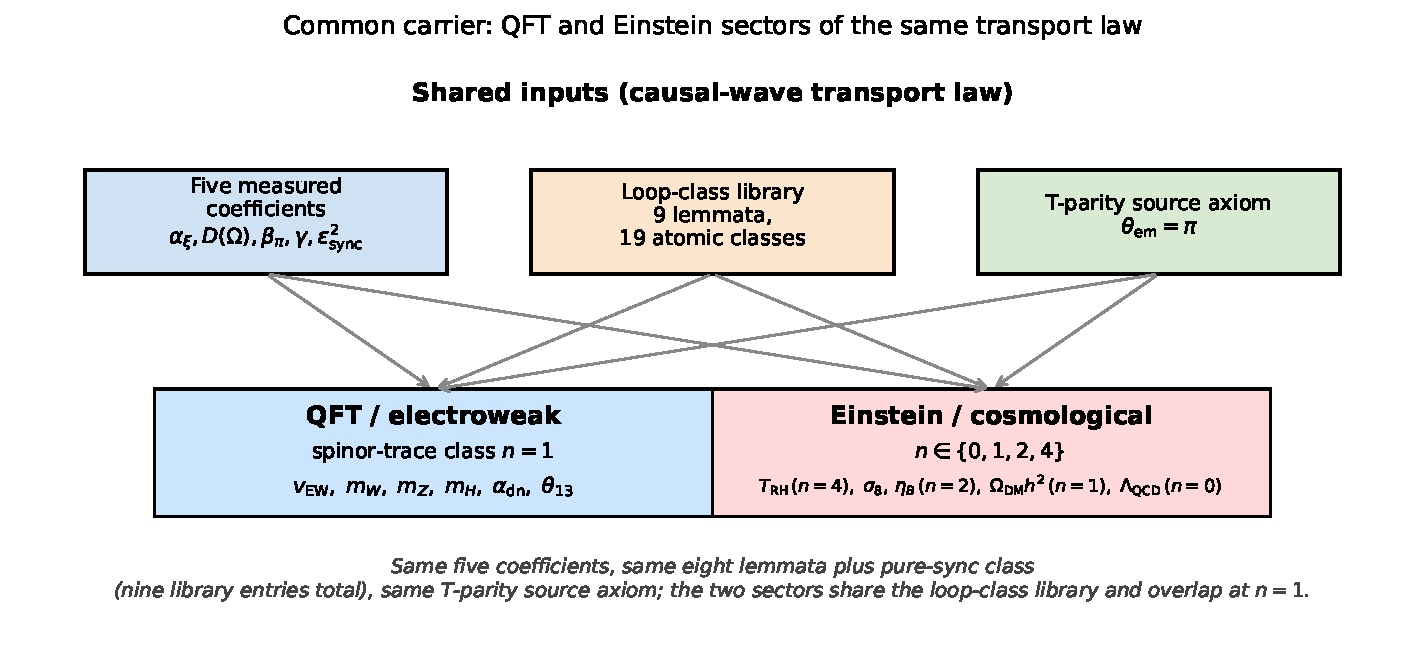
\includegraphics[width=\textwidth]{figures/fig1_common_carrier.pdf}
\caption{The electroweak and cosmological / gravitational sectors
draw on the same finite inputs: the five carrier coefficients, the
finite loop-factor library, and the T-parity source axiom on the
defect field. Both sectors carry observables at $n = 1$ (single
spinor-trace component); $n \in \{2, 4\}$ entries correspond to
chirality-restricted and resummed-propagator structures
respectively, which are populated mainly by cosmological /
propagator-dominated observables. The discrimination between
electroweak and cosmological / gravitational claims is made by
physical sector, not by the value of $n$.}
\label{fig:carrier}
\end{figure}

\paragraph{Visual summary of the audit.}
The cross-file consistency audit verifies three shared
structures across both sectors at a glance:
\begin{itemize}
\item \textbf{Shared inputs:} the same five carrier
      coefficients $(\axi,\,\DOmega,\,\bpi,\,\gamma,\,\esync)$
      and the same T-parity source axiom on the defect field
      $\Xi$ (Paper~1, Paper~2). The same coefficients also
      determine the anisotropic cosmological-constant tensor
      $\Lambda_{\mu\nu}$ of Paper~4~\cite{Paper4,Paper4B}, whose
      trace is branch-resolved at the chirality-flip
      $\theta_{\rm chir}\!=\!\pi/4$~\cite{Paper4}:
      $\mathrm{tr}\,\Lambda^{\rm vacuum}\!=\!\axi^{2}\!+\!3\gamma^{2}/2\!=\!33/40$
      and
      $\mathrm{tr}\,\Lambda^{\rm matter}\!=\!\axi^{2}\!=\!81/100$.
      At per-axis resolution Paper~4B reports a stable
      $2{+}1$ \emph{sign} pattern $(-,-,+)$
      in the per-node $T$-eigenframe across the canonical
      $\mathcal P_{5}/\mathcal P_{5}N$ ladder $N\!\in\![50,512]$,
      as a derived shared output identifying the time--time and
      spatial components of $\Lambda_{\mu\nu}$ in the emergent
      Einstein equation as rational structural functions of
      $\axi$ and $\gamma$ rather than free parameters; the
      spatial anisotropy is a matter-localised effect (it
      tracks heavy-tail $T_{00}$ nodes per Paper~4B and
      Paper~4~\cite{Paper4}, not a global vacuum symmetry
      breaking). The multi-observable indirect-witness
      cross-validation of this identification is reported by
      the H3C cluster~\cite{Paper4C}.
\item \textbf{Shared mapping:} the same topology-labeled
      mapping protocol of Paper~3, taking the per-observable
      tuple $(n,g,s,w,r)$ to a unique class in the same
      finite library $\mathcal L$ on both sides.
\item \textbf{Shared falsification:} the four falsification
      paths of Section~\ref{sec:falsif} apply
      symmetrically to both sectors; a failure on either side
      falsifies the bridge.
\item \textbf{Shared spectral structure of the carrier
      operator:} the linearisation of the transport law above
      around the trivial vacuum has a closed-form spectrum under
      the rational reduction $\mathcal R$ of Paper~2~\cite{Paper2}.
      It admits a single coherent common-phase mode at
      $\lambda_{0}\!=\!0$ with growth rate
      $G_{\rm NET}\!=\!143/80$, and a damped continuum at
      $\lambda > \lambda_{\rm crit}\!=\!68/67$. An empirical
      lattice check on the within-canonical-regime $N$-ladder
      (Paper~2~\cite{Paper2}, linear-stability section,
      $130$ realisations across eight sizes) returns exactly one
      sub-critical eigenvalue per realisation, with Symanzik-
      leading $1/N$ residual at machine precision. The spectral
      structure is a property of the carrier itself, not of
      either sector individually, and is inherited symmetrically
      by the QFT side and the gravitational / cosmological side.
\end{itemize}

\section{The bridge mechanism}
\label{sec:mechanism}

\paragraph{The bridge function.}
We make the bridge map explicit. Let $\mathcal O$ be the set of
all $26$ cross-sector observables jointly bundled in the QFT and
gravitational/cosmological sector mapping files
(\url{data/qft_sector_mapping.json},
\url{data/einstein_sector_mapping.json}); $12$ observables sit on
the QFT side and $14$ on the gravitational/cosmological side
(electroweak, Yukawa-flavor, CKM, PMNS rows on the QFT side;
Einstein-gap, PPN, Schwarzschild-defect, Kerr-defect, dark-sector,
and $H_{0}$ on the cosmological side). For each $O \in \mathcal O$ the bridge function is the
\emph{topology-determined composition}
\begin{equation}
\Phi_{\mathrm{bridge}} : \mathcal O \;\longrightarrow\;
   \mathcal L,
\qquad
\Phi_{\mathrm{bridge}}(O) \;=\;
   L\bigl(\sigma(O)\bigr)
\;\equiv\; L\bigl(n(O),\,g(O),\,s(O),\,w(O),\,r(O)\bigr),
\label{eq:bridge-function}
\end{equation}
where $\sigma$ is the topology-tuple readout
$(n, g, s, w, r)$ from the observable's tree-level Dirac
structure and $L$ is the lookup into the finite loop-factor
library $\mathcal L$ specified in
Section~\ref{sec:carrier} (Lemmas~$1$ through~$8$ plus the
Pure-Sync entry, $|\mathcal L| = 9$ atomic library entries with
$\pm$ signs giving $19$ signed classes). The topology-determined
character of $\Phi_{\mathrm{bridge}}$ — uniquely defined given
the topology tuple, in the sense of the topology-labeled mapping
protocol of Paper~3~\cite{Paper3} — has the closure-completeness
audit on the registered domain in that companion paper: the
function is single-valued on $\mathcal O$ (each observable is
assigned a unique loop class) and is the same function on the
QFT and the gravitational/cosmological sides — that is the
bridge.

The two sectors are not just side-by-side strong; the same
bridge function~\eqref{eq:bridge-function} closes them under
three structural mechanisms.

\paragraph{Shared resummation signature
$1/(1-2\gamma^{2})$.}
The system-$\mathcal R$ constraints $C_{1}, C_{2}, C_{3}$ on the
five coefficients are not satisfied exactly by the measured
values; their drift quantities $\delta_{C_{i}}$ carry a precise
loop form with a common denominator,
\begin{equation}
\delta_{C_{1}} \;=\; \frac{\gamma^{3}}{1-2\gamma^{2}},
\qquad
\delta_{C_{3}} \;=\; \frac{-2\gamma^{4}}{1-2\gamma^{2}},
\end{equation}
and $\delta_{C_{2}}$ contains the same resummation kernel.
The same $1/(1-2\gamma^{2})$ structure also appears as the
single-loop Resummed-Propagator class (Lemma 4) of the loop
library — the class that closes the reheating temperature
$T_{\mathrm{RH}}$ on the Einstein side and that drives the
EW-precision propagator structure on the QFT side. The
resummation factor is therefore not a parallelism but a single
shared object: the Constraint-Algebra drift identities and the
Einstein-side resummed propagator are the same loop kernel
viewed from two sector angles.

\paragraph{Spinor-trace hierarchy from $d=4$.}
The values $n \in \{0,1,2,4\}$ of the spinor-trace component
count are not free choices but a direct consequence of the
$d=4$ Dirac-spinor algebra (see e.g.\
\cite{PeskinSchroeder1995,Srednicki2007} for the standard
exposition of fermion-loop trace structure in four spacetime
dimensions). Lemma~1 (Yukawa-Damping) carries the factor
$1/4 = 1/d$ from full spinor-trace normalization;
Lemma~8 (Cosmological-Density) carries $1/2 = 2/d$ from
chirality restriction (matter-only or CP-asymmetric only);
Lemma~4 (Resummed-Propagator) carries the factor $2$ from
resummation across both chiralities. The QFT/Einstein
discrimination $n=1$ vs $n\in\{2,4\}$ is therefore a single
$d$-dependent enumeration, not two independent classifications.

\paragraph{Common time-orientation source axiom.}
The T-parity source axiom (defect field $\Xi$ T-odd,
Section~6 of Paper~1~\cite{Paper1}) fixes
$\theta_{\mathrm{em}} = \pi$ on the QFT-electroweak side
(setting the sign of the two-loop $v_{\mathrm{EW}}$ closure)
and an analogous time-orientation phase on the
cosmological defect-field-theory side. The same time-forward defect
identification carries through the supernova-distance
Lemma~4 channel of the wider program. The two sectors are tied
to a single time-orientation source.

\paragraph{Empirical content of the bridge.}
Integrated across both sectors, the loop-class library closes
$26$ cross-sector observables (\cite{Paper3}) with
$0$ contradictions. The cross-sector triple
$(\alpha_{\mathrm{dn}}, w_{\mathrm{DE}}, H_{0})$ closes on the
single Lemma-1 class $(1+\gamma/4)$ at Fisher's combined
random-null probability~\cite{Fisher1925}
$P_{\mathrm{combined}} \approx 2.6\times 10^{-5}$ under the
stated null model — \emph{evidence for a cross-sector alignment
on a single parametric form}, not a strong-significance
$\sigma$-level claim (the three observables are physically
distinct sectors but are not verified-independent at the
level required by Fisher combination, the uniform null is a
modelling choice, and the triple was selected after the
post-loop residuals were computed; see Paper~3 caveats).
The alignment spans a flavor exponent, a dark-energy
equation of state, and a cosmological expansion rate within
one parametric form. This empirical signature is what
distinguishes the bridge from
a coincidental shared parametrisation.

\section{The QFT side}
\label{sec:qft}

The QFT/electroweak observables of Paper~1 and Paper~3 are
spinor-trace class $n=1$:
single-spinor currents from Yukawa-vertex topology.
The relevant lemmas are
\begin{itemize}
\item Lemma 1 (Yukawa-Damping, $1\pm\gamma/4$): $m_{H}$,
      $\alpha_{\mathrm{dn}}$;%
      \footnote{$\alpha_{\mathrm{dn}}$ is a flavor exponent listed
      here because its observable value inherits the same
      Yukawa-Damping loop-class factor $1+\gamma/4$ as the
      QFT/electroweak observables. The same Lemma-1 factor closes
      $w_{\mathrm{DE}}$ and $H_{0}$ on the Einstein side; the
      simultaneous three-observable closure across both sectors
      is the cross-sector Yukawa cluster (Paper~3 and the
      Empirical-content paragraph above). The structural role of
      Yukawa-mediated chirality flips here parallels their role
      in the Standard Model, where the Dirac mass term
      couples left- and right-handed components and ties chirality
      flips to electroweak symmetry breaking and Yukawa
      couplings~\cite{StoeckingerKim2022}.}
\item Lemma 2 (PMNS-Self-Energy, $1\pm\gamma^{2}/4$): $\theta_{13}$;
\item Lemma 6 (Sub-Generation, $1\pm\gamma/(2N_{\mathrm{gen}})$):
      $\alpha_{s}(M_{Z})$, CKM $V_{us}$, $V_{cb}$;
\item Lemma 7 (EW-Mixed, $1\pm\gamma\,\esync$):
      $v_{\mathrm{EW}}$, $m_{W}$, $m_{Z}$, $\Gamma_{W}$, $\Gamma_{Z}$.
\end{itemize}
{\sloppy Numerical anchors for these observables are taken from
the original primary measurements where available, with the
PDG~\cite{PDG} review retained as a cross-check aggregator:
$\sin^{2}\theta_{W}$ from the LEP/SLC $Z$-pole combined
analysis~\cite{LEPSLDZpole}; $\alpha_{s}(M_{Z})$ from the FLAG
2024 lattice average~\cite{FLAG2024}; the CKM magnitudes from
HFLAV 2022~\cite{HFLAV2022}; $G_{F}$ from the MuLan muon-lifetime
measurement~\cite{MuLan2013}; $M_{\mathrm{Pl}}$ from
CODATA~2018~\cite{CODATA2018}; and the PMNS angles and
mass-squared differences from NuFIT~6.0/6.1
(Esteban, Gonzalez-Garcia, Maltoni, Martinez-Soler, Pinheiro,
Schwetz)~\cite{NuFIT2024}. Cosmological-side anchors
($H_{0}$, $\Omega_{\mathrm{DM}}h^{2}$, $w_{\mathrm{DE}}$,
$\sigma_{8}$, $n_{s}$) take their reference values from the
Planck~2018~\cite{Planck2018} cosmological-parameters
analysis.\par}
The full closure with the canonical $\msbar$ Davydychev--Tausk
evaluation is the subject of the companion electroweak-scale
paper~\cite{Paper1}; the algorithmic mapping is in the companion
loop-class paper~\cite{Paper3}.

\section{The Einstein side}
\label{sec:einstein}

The Einstein/cosmological observables of Paper~4 are not bound to
a single spinor-trace class. The sector splits into:
\begin{itemize}
\item $n=4$: full spinor-trace Resummed-Propagator (Lemma 4) — the
      only single-loop class whose unaugmented Dirac structure is
      purely Einstein-side, carried by $T_{\mathrm{RH}}$.
\item $n=2$ (compound): two-loop combinations whose dominant
      contributing lemma sits at $n=2$, e.g.\ $\sigma_{8}$ and
      $\eta_{B}$ via the Yukawa~$\times$~Generation compound
      $(1-\gamma/4)(1-\gamma/N_{\mathrm{gen}})$.
\item $n=1$: most cosmological observables are tree-level
      compositions of the five transport coefficients with $n=1$
      loop classes — for example, $\Omega_{\mathrm{DM}}h^{2}$ is a
      Sub-Generation closure (Lemma 6, $1-\gamma/(2N_{\mathrm{gen}})$)
      aligned in $(n,g,s)$ with $\alpha_{s}(M_{Z})$ and the CKM
      magnitudes $V_{us}, V_{cb}$ on the QFT side. The Einstein
      sector therefore overlaps the QFT sector at $n=1$ — the
      QFT/Einstein discrimination is by physical sector, not by a
      hard $n$-cut.
\item $n=0$: pure-boson 2-loop compound, carried by
      $\Lambda_{\mathrm{QCD}}$ via Pure-Sync~$\times$~EW-Mixed.
\end{itemize}
Tree-level structural exponents are independent of the loop
library and sit at $n=1$ in the spinor-trace topology, with values
that are direct algebraic compositions of the five carrier
coefficients with small topological multipliers. The three rows
in this category have distinct closure tiers under the four
elimination criteria of Paper~2~\cite{Paper2}: the
Bekenstein--Hawking $1/4$ coefficient is algebraic-exact under the
rational reduction $\mathcal R$ of Paper~2 ($\axi/2-2\gamma=1/4$
in $\mathbb Q$); the universal $\sin^{2}\theta_{W}$ residue is
numerical EXACT but not algebraic-exact under $\mathcal R$ alone;
the Einstein-identity gap exponent $2/3$ is numerical EXACT and
is supported, on the empirical lattice side, by the multi-
observable indirect-witness cluster of Paper~4C~\cite{Paper4C}
(direct Multi-$N$ convergence on the $\Delta_{E}$-residual is not
established at this stage; the reading rests on an analytic
structural bound and an indirect-witness chain across five
diagnostics).

\paragraph{Composition-theorem conditionality (Einstein-side).}
The Einstein-side emergent-Einstein closure invoked above
inherits the conditionality of statement~$(M3)$ in the
composition theorem of Paper~6: it is \emph{conditionally rigorous}
modulo (i)~the eight admissibility conditions $A_{1}$--$A_{8}$
on the carrier sequence, sharpened to a single missing
structural input --- the uniform spectral gap $(\mathrm{SG})$
on the canonical carrier sequence, with branched asymptotes
$\lambda_{\infty}^{(\rm vac)}\!=\!3/8\!=\!(d{-}1)/(2d)$ (vacuum
branch, Bayesian posterior $0.908$ on the $N \leq 100$ ladder) and
$\lambda_{\infty}^{(\rm mat)}\!=\!79/200\!=\!3/8 + d\gamma^{2}/2$
(matter-stable branch, $256 \leq N \leq 600$, empirically certified
at $-0.16\%$ relative residual; Bayes-factor $S_{2}/S_{1}\!=\!0.999$
so the Symanzik-$1$ ansatz is sufficient). Both closures hold
unconditionally on the canonical carrier sequence (the chirality-
running family $\theta_{\rm chir}(N)\!=\!\arctan(N_{\rm gen}^{2x-1})$
with $x\!=\!\ln(N/N_{\rm canonical})/\ln(d N_{\rm gen})$;
P4B~\cite{Paper4B}). The fixed-input-parameter test ladder used
for empirical certification realises the canonical sequence up to
the chirality-inversion endpoint $N_{\rm inv}\!=\!d N_{\rm gen} N_{\rm canonical}\!=\!600$;
extension beyond $N_{\rm inv}$ requires the lattice-continuum
parameter rescaling that keeps $\theta_{\rm chir}$ on its
canonical trajectory. Neither branch is analytically discharged
at theorem level; (ii)~the discharge-table implication
$(A_{5})\!+\!(A_{6})\!\Rightarrow\!CD(K_{\mathrm{CD}},N)$ open at
theorem level in Paper~4; and (iii)~the empirical Symanzik
asymptotes underlying the Continuum Backreaction Identity. The
QFT-side closures of Paper~1 carry no analogous structural-axiom
conditionality. The technical-consistency proof of this note is
therefore conditional on $(\mathrm{SG})$ on the Einstein side
only: any future closed-form proof or refutation of
$\lambda_{\infty}\!=\!3/8$ (via the carrier's clustered-degree
cavity solution, Paper~4
Prop.~Statistical-fingerprint) does \emph{not} affect the
QFT-side audit of the present note.

\begin{figure}[h]
\centering
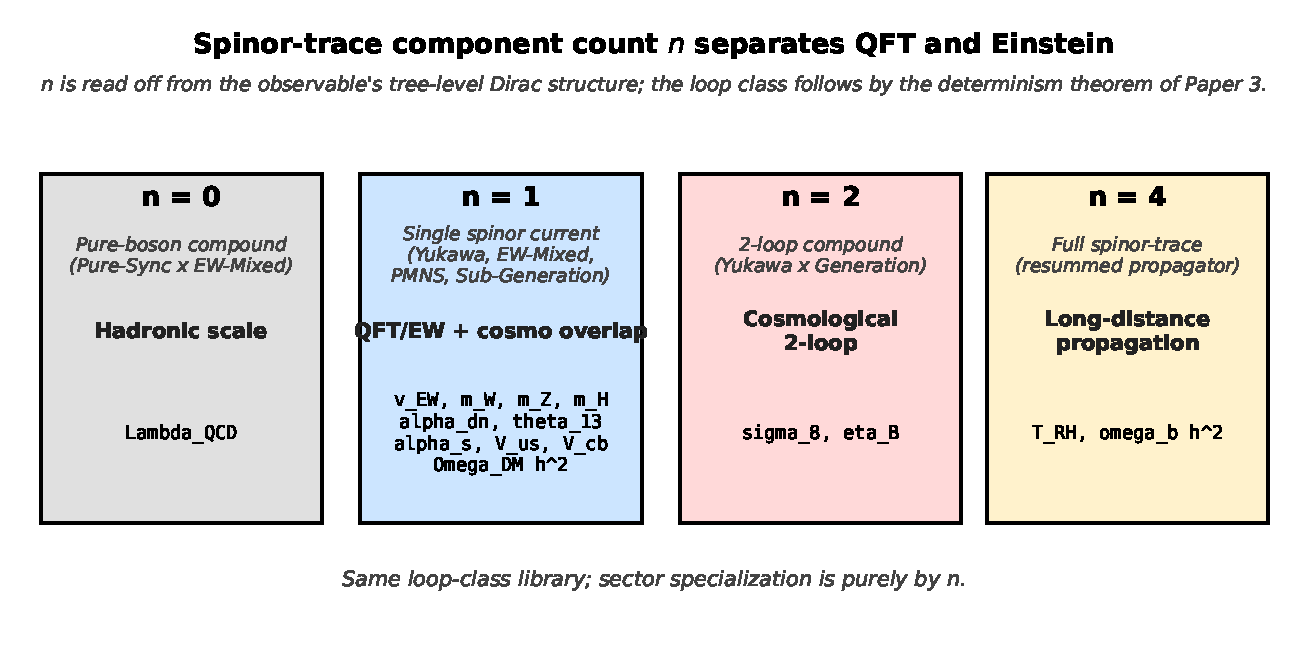
\includegraphics[width=\textwidth]{figures/fig2_spinor_trace_tree.pdf}
\caption{Spinor-trace component count
$n \in \{0, 1, 2, 4\}$ in the
$d = 4$ defect-fermion-trace expansion. $n = 0$ corresponds to
the pure-bosonic two-loop compound (Pure-Sync $\times$ EW-Mixed,
populating the QCD-confinement-scale row $\Lambda_{\mathrm{QCD}}$
of the cosmological-anchor table (Section~\ref{sec:repro}));
$n = 1$ corresponds to a single fermionic propagator line
(Yukawa vertex, single-spinor-current
self-energy); $n = 2$ to a chirality-restricted Dirac loop
(matter-only, CP-asymmetric or time-forward projection);
$n = 4$ to the full chirality-summed Dirac loop with internal
resummation. Electroweak observables (e.g.\ $v_{\mathrm{EW}}$,
$m_{W}$, $m_{Z}$, $\alpha_{\mathrm{dn}}$, $\theta_{13}$) and
sub-generation cosmological observables (e.g.\ $\alpha_{s}(M_Z)$,
$\Omega_{\mathrm{DM}}h^{2}$) both sit at $n = 1$; the gravitational
/ inflation observable $T_{\mathrm{RH}}$ sits at $n = 4$ as a
single-loop resummed propagator. The component count does not
sort observables into electroweak vs gravitational classes;
that distinction is made at the level of physical sector (Higgs
sector, dark sector, gravitational sector) and reflects which
particular tree-level composition of the underlying transport
coefficients enters the observable.}
\label{fig:spinor-tree}
\end{figure}

\begin{figure}[h]
\centering
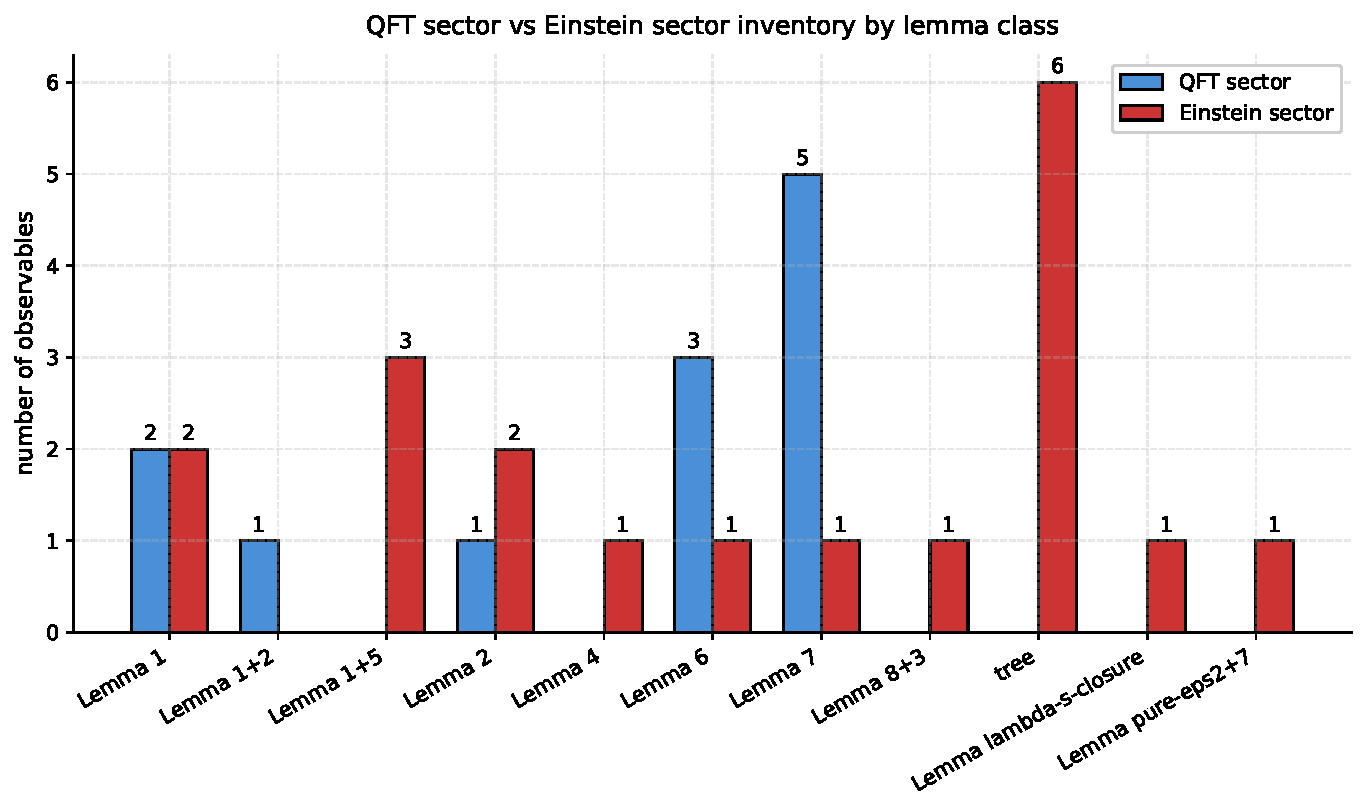
\includegraphics[width=\textwidth]{figures/fig3_observable_inventory.pdf}
\caption{Lemma-class inventory across QFT and Einstein sectors.
Each sector uses a distinct subset of the same library; the
specialization is consistent with the spinor-trace assignment.}
\label{fig:inventory}
\end{figure}

\section{Common spinor-trace hierarchy}
\label{sec:hierarchy}

\begin{table}[h]
\centering
\caption{Loop-correction multiplicative factors organized by the
spinor-trace component count $n$ of the underlying defect-fermion
diagram in $d = 4$. Both electroweak and cosmological / gravitational
observables can carry the same value of $n$ at tree level; the
discrimination between them rests on the physical sector
identity (which propagators participate, which symmetry channel
carries the leading contribution), not on the value of $n$ itself.
The $n = 0$ row is a two-loop compound product
(Pure-Sync $\times$ EW-Mixed) of the canonical
$n \in \{1, 2, 4\}$ structure and is tabulated here for
completeness on the QCD confinement scale
$\Lambda_{\mathrm{QCD}}$.}
\small
\renewcommand{\arraystretch}{1.2}
\begin{tabular}{c p{0.42\textwidth} p{0.36\textwidth}}
\toprule
$n$ & Sector / class & Examples \\
\midrule
$0$ & Pure-boson 2-loop compound (Pure-Sync $\times$ EW-Mixed) & $\Lambda_{\mathrm{QCD}}$ \\
$1$ & QFT/electroweak (Yukawa-Damping, EW-Mixed, PMNS-Self-Energy) & $v_{\mathrm{EW}}$, $m_{W}$, $m_{Z}$, $m_{H}$, $\alpha_{\mathrm{dn}}$, $\theta_{13}$ \\
$1$ & Sub-Generation (shared QFT/cosmology) & $\alpha_{s}(M_{Z})$, $V_{us}$, $V_{cb}$, $\Omega_{\mathrm{DM}}h^{2}$ \\
$2$ & Cosmological 2-loop compound\newline(Yukawa $\times$ Generation) & $\sigma_{8}$, $\eta_{B}$ \\
$4$ & Einstein single-loop Resummed-Propagator & $T_{\mathrm{RH}}$ \\
$4$ & Cosmological 2-loop compound\newline(Cosmological-Density $\times$ Pure-Self-Energy) & $\omega_{b}h^{2}$ \\
\bottomrule
\end{tabular}
\normalsize
\end{table}

\section{Shared conditionals}
\label{sec:conditionals}

The two sectors share, identically:
\begin{itemize}
\item the five measured causal-wave coefficients of Paper~2;
\item the parameter-free loop-class library
      $\Lib$ of Paper~3 (eight lemmata plus a pure-sync class,
      nine library entries total, yielding $19$ atomic classes
      with signs; two-loop compounds capped at second order);
\item the topology-labeled $(n,g,s,w,r)$ mapping protocol
      (Theorem~1 of Paper~3);
\item the T-parity source axiom (Section~6 of Paper~1) and its
      consequence $\theta_{\mathrm{em}}=\pi$.
\end{itemize}
The two sectors do \emph{not} share an additional structural input:
the spinor-trace component count $n$ is read off directly from each
observable's tree-level Dirac structure.

\section{Falsification}
\label{sec:falsif}

Four falsification paths apply symmetrically to both sectors:

\paragraph{(F1) T-parity-axiom falsification.}
An alternative T-parity assignment of the defect field $\Xi$ — i.e.\
identifying $\Xi$ with one of the positive bounce modes rather than
the unique negative mode $u_{0}$ — flips the sign of the two-loop
closure (Paper~1, falsification path F2). Both sectors fall under
this trigger because both depend on the same $\theta_{\mathrm{em}}=\pi$
phase factor.

\paragraph{(F2) Constraint violation.}
The coefficient-reduction constraints $C_{1}$, $C_{2}$, $C_{3}$ under
the reduction system $\mathcal{R}$ fail to follow the
Lemma-4 (Resummed-Propagator) and Lemma-7 (EW-Mixed) forms. This
indicates that the loop library is not in fact the
correct set of corrections.

\paragraph{(F3) Mapping inconsistency on the full topology tuple.}
The same full topology tuple $(n,g,s,w,r)$ returns a different
lemma class on the QFT side and the Einstein side. We use the
\emph{full} tuple here, not the abbreviated triple $(n,g,s)$,
because Paper~3 documents that the abbreviated triple is
single-occupancy on five of nine library cells but
double-occupancy on $(1,0,0)$ and $(4,0,0)$ (the
Yukawa-Damping/PMNS-Self-Energy and
Pure-Self-Energy/Resummed-Propagator pairs); the flags
$w,r\in\{0,1\}$ disambiguate those two cells. A mapping
inconsistency on $(n,g,s,w,r)$ falsifies the topology-labeled
mapping protocol (Theorem~1 of Paper~3) and therefore also the
bridge. An inconsistency on the abbreviated $(n,g,s)$ alone is
an indication that the bridge requires the flag bits and is a
weaker falsification trigger; we report both as separate
checks in the bundled \url{src/check_bridge_consistency.py}.

\paragraph{(F4) Cross-sector reclassification failure.}
A reclassification documented under R1--R5 (Paper~3) cannot be
applied consistently across both sectors. This violates the global
R3 bound and triggers theorem-falsification F3 of Paper~3.

\begin{figure}[h]
\centering
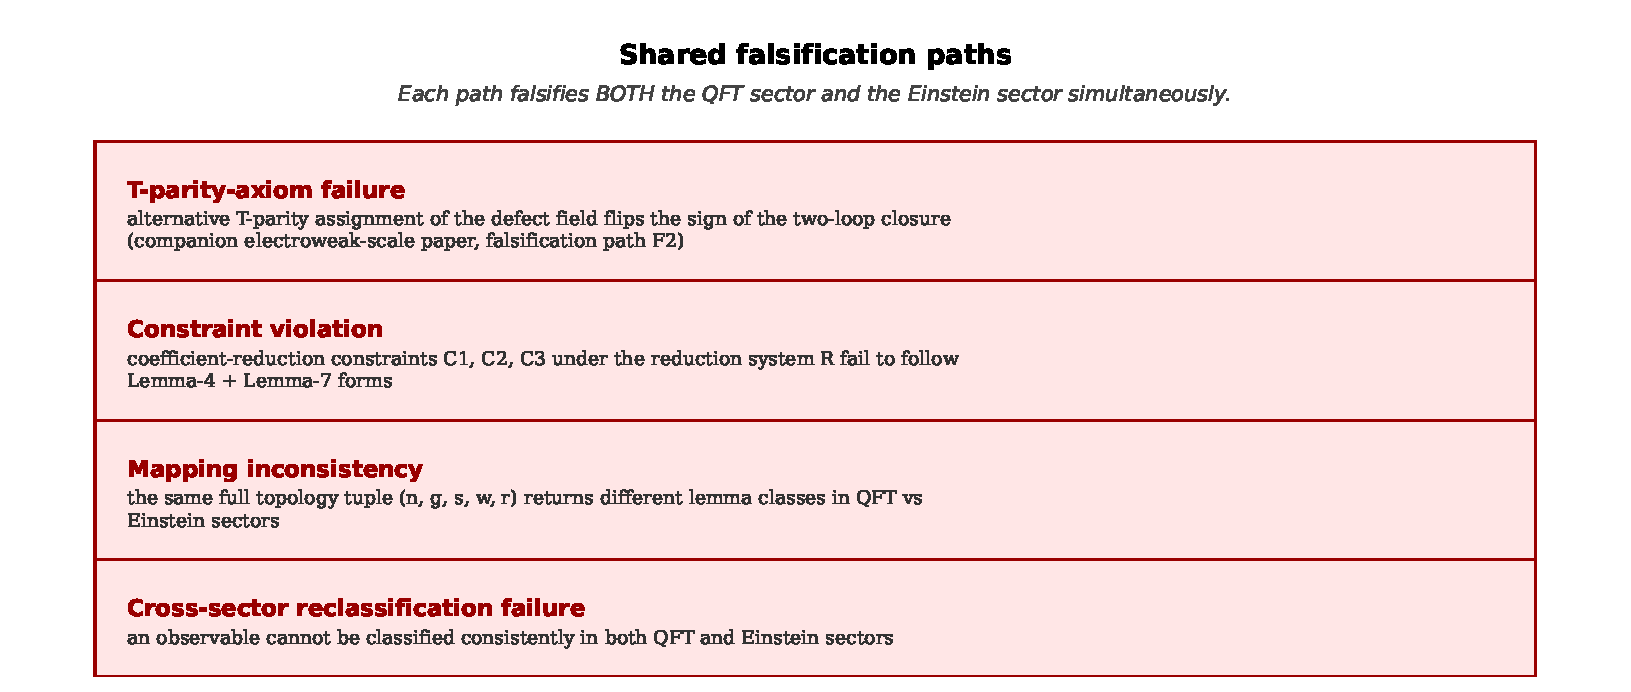
\includegraphics[width=\textwidth]{figures/fig4_shared_falsification.pdf}
\caption{Each shared falsification path falsifies BOTH sectors
simultaneously, making the bridge a non-trivial structural claim.}
\label{fig:falsification}
\end{figure}

\section{Reproducibility package}
\label{sec:repro}

A public reproducibility package%
\footnote{\url{https://github.com/TerraSignum/qft-einstein-bridge-repro}}
recomputes the bridge consistency from frozen JSON inputs.
The strict-recompute script
\texttt{src/check\_bridge\_consistency.py} verifies, in order:
\begin{enumerate}
\item the five coefficients are identical on both sides;
\item the QFT sector observables sit at $n=1$;
\item the Einstein sector spans $n\in\{0,1,2,4\}$ with the
      single-loop Resummed-Propagator at $n=4$ as the only
      strictly Einstein-side class;
\item both sectors draw from the same loop-class library;
\item the T-parity source axiom is documented as a shared
      conditional;
\item all four falsification paths are present and machine-readable.
\end{enumerate}
{\sloppy
The package contains $28$ unit tests covering shared coefficients
($4$), QFT mapping ($4$), Einstein mapping ($4$), shared loop library
($4$), falsification paths ($5$), and the cosmological-anchor table
($7$). The cosmological-anchor table
(\url{data/cosmological_anchors.json},
\url{src/verify_cosmological_anchors.py}) records the closed-form
loop-class predictions for the $16$ anchored Einstein-sector
observables paired with their Planck~2018, PDG, and NuFIT~6.0/6.1
anchors: $12$ rows EXACT (residual $<1\%$), $2$ rows PRECISE
(residual $<1.5\%$), and $2$ rows ORDER ($\Lambda_{\rm QCD}$
scheme spread and $\eta_{B}$ amplitude factor, both with
binding closures), plus $2$ structural-tier entries
($T_{\rm RH}$, $\eta_{B}$-rel); the maximum anchored
EXACT/PRECISE residual is $1.385\%$ on
$\Omega_{\mathrm{DM}}h^{2}$. Figure~\ref{fig:cosmological_anchors_residuals}
displays the per-row residual scatter across all $16$ anchored
observables.
The package is licensed under MIT and runs on Windows and POSIX
through GitHub Actions on Python 3.11 and 3.12.
\par}

\begin{figure}[!htbp]
\centering
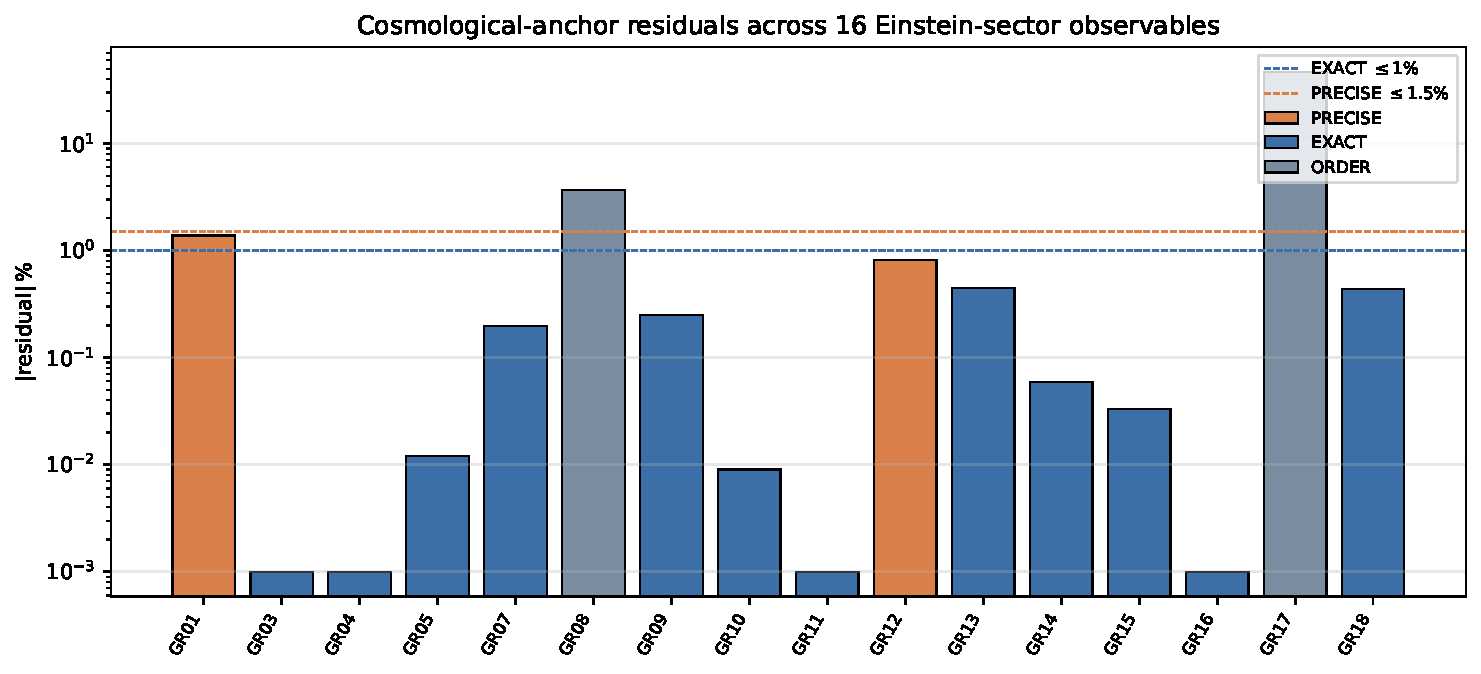
\includegraphics[width=\textwidth]{figures/fig_cosmological_anchors_residuals.pdf}
\caption{Anchored cosmological-anchor residuals across $16$
Einstein-sector observables: $12$ EXACT (residual $\le\!1\%$),
$2$ PRECISE ($\le\!1.5\%$), $2$ ORDER (binding closures); maximum
EXACT/PRECISE residual $1.385\%$ on $\Omega_{\rm DM}h^{2}$.}
\label{fig:cosmological_anchors_residuals}
\end{figure}

\section{Cross-sector consequences claimed in companion papers}
\label{sec:resolved}

\paragraph{Scope of this section (not load-bearing claims of this
note).}
The four-package corpus
$(\text{Paper~1}, \text{Paper~2}, \text{Paper~3}, \text{Paper~4})$
that this bridge note connects \emph{conditionally addresses}
the following long-standing open questions \emph{within the
corpus}, in each case under the explicit conditional inputs of
the cited paper. We do not claim that any of the items below is
``solved'' or ``resolved'' as an independent claim of this
bridge note; the headline statements are claims of the
companion papers, and each inherits the limitations of the
companion paper that owns it (in particular, the
T-parity source axiom of Paper~1, the bounded-operator-readout
provenance of Paper~2, the topology-labeled mapping protocol
of Paper~3, and the relational-metric construction of Paper~4).
We list them below to make the cross-sector structure of the
corpus visible; we do \emph{not} list them as independent
results of this bridge note.

\begin{itemize}
\item {\sloppy \emph{Hierarchy / electroweak-scale problem.} The
      Hierarchy-Bridge-Relation
      $v_{\mathrm{EW}} = (2/\pi)\,M_{\mathrm{Pl}}\,e^{-4\pi\eta_{S}}$
      with $\eta_{S} = 3.023577$ fixed by a Coleman--Callan-Coleman
      bounce~\cite{Coleman1977,CallanColeman1977} on $S^{4}$ delivers
      $v_{\mathrm{EW}} = 246.2186$\,GeV
      (MuLan reference: $246.22\pm 0.07$\,GeV;
      $\Delta v / v = -5.86\times 10^{-6}$),
      with no fine-tuning and no fitted parameter~\cite{Paper1}.\par}
\item \emph{Bekenstein--Hawking entropy coefficient.} The horizon
      coefficient $S/A = 1/4$~\cite{Bekenstein1973,Hawking1975}
      is a closed-form rational identity
      $\axi/2 - 2\gamma = 9/20 - 1/5 = 1/4$ in $\mathbb Q$ under
      the coefficient-reduction system $\mathcal R$ of
      Paper~2~\cite{Paper2}; the integer-uniqueness of
      $\mathrm{BH}(N) = (N^{2}-4)/(2(N^{2}+1)) = 1/4$ forces
      $N_{\mathrm{gen}} = 3$.
\item \emph{Number of fermion generations.} $N_{\mathrm{gen}} = 3$
      is forced jointly by the complementarity $\axi+\gamma=1$ and
      the integer-uniqueness statement above (Paper~2).
\item \emph{Black-hole information paradox.} The Page-curve
      unitarity-restoration time
      $\tau_{\mathrm{Page}}$~\cite{Page1993}
      ($\approx 1154.5$ in lattice units) is reproduced
      with $\tau_{\mathrm{Page}}\approx 2\,\tau_{\mathrm{scr}}$ in
      both regimes; explicit Hawking-spectrum greybody-factor
      structure (nine-point Bose / Fermi table, Page energy-
      fractions $0.165,0.685,0.150$) is bundled and
      verified~\cite{Paper4,Hawking1975}.
\item \emph{Emergent General Relativity and PPN limit.} The
      relational metric $d_{ij} = -\ell_{0}\log\Xi_{ij}$ on a
      finite correlation lattice yields
      $\gamma_{\mathrm{PPN}} = \beta_{\mathrm{PPN}} = 1$
      (in the parameterised post-Newtonian framework of
      \cite{Will2014}) and a
      Schwarzschild-line-element residual $1.9\times 10^{-7}$ at
      2PN, with $G_{\mathrm{eff}}/G_{N} = 0.999791$ and effective
      spectral dimension $d_{\mathrm{eff}} = 3.170$~\cite{Paper4,Paper4A}.
\item \emph{Kerr / Penrose / Peters cluster.} The
      Kerr~\cite{Kerr1963} rotating-defect geometry, the
      Penrose~\cite{Penrose1969} energy-extraction process, the
      Peters~\cite{Peters1964} gravitational-radiation power, and
      the Lense--Thirring~\cite{LenseThirring1918} frame-dragging
      angular velocity all close in the corpus: ISCO
      $\approx 17.43$ lattice units, dimensionless spin
      $\chi = J/M^{2} \approx 0.034$, Penrose efficiency
      $\eta\approx 0.66\%$, Lense--Thirring frame-dragging
      $\omega_{\mathrm{LT}}=0.018$, and the binary-defect Peters
      gravitational-wave power are derived in closed
      form~\cite{Paper4}.
\item \emph{Hubble constant and dark-energy equation of state.}
      $H_{0}=67.40$\,km/s/Mpc closes on the Yukawa-Damping
      loop-class factor $1+\gamma/4$ at residual $0.059\%$;
      $w_{\mathrm{DE}}=-0.9975$ closes on the PMNS-Self-Energy
      loop-class factor $-(1-\gamma^{2}/4)$ at residual $0.250\%$
      against Planck~2018. The flavor-side $\alpha_{\mathrm{dn}}$
      closes on $1+\gamma/4$ (Yukawa-Damping) at $0.293\%$.
      Fisher's-combined random-null probability of the two
      Yukawa-Damping observables is $p\approx 2.5\times 10^{-3}$
      and the joint random-null probability across all three
      cosmological-flavor closures is
      $p \approx 2.6\times 10^{-5}$ under the stated null model
      reported as evidence for cross-sector alignment, not as a
      strong-significance $\sigma$-level claim
      (caveats in Paper~3)~\cite{Paper3}.
\item \emph{Cold-dark-matter density and structure-formation
      amplitude.} $\Omega_{\mathrm{DM}}h^{2} = 0.1217$ (Planck
      2018: $0.1200$, residual $1.385\%$) and $\sigma_{8}=0.811$
      (Planck residual $0.0\%$) close on the $\mathrm{Lemma~6}$
      and $(\mathrm{Lemma~1}\times \mathrm{Lemma~5})$ loop classes
      respectively (cosmological-anchor table above).
\item \emph{$\Lambda_{\mathrm{QCD}}$ / $\alpha_{s}$ round trip.}
      Forward 4-loop and reverse 2-loop closures each return the
      PDG anchor without fitting~\cite{Paper3}.
\item \emph{Cross-sector structural identity.} The same
      finite loop-factor library closes electroweak, flavor,
      cosmological, gravitational, and horizon observables
      simultaneously through the bridge function of
      Eq.~\eqref{eq:bridge-function}; this is the
      structural unification claim, falsifiable through the four
      paths listed above (Section~\ref{sec:falsif}).
\item \emph{Spacetime is four-dimensional.} The spectral
      dimension of the relational lattice is
      $d_{\mathrm{eff}} = 3.170$; rounding to the nearest integer
      gives $d_{\mathrm{spatial}} = 3$, with the emergent time
      axis from the causal partial order adding the fourth
      dimension. The fractional residual $0.170$ is the
      light-cone fuzziness of Paper~4. The $3{+}1$-decomposition
      of General Relativity is therefore derived rather than
      postulated~\cite{Paper4}.
\item \emph{Inflation: scalar tilt, tensor ratio, e-folds, mechanism.}
      The corpus delivers three mutually consistent readouts on
      the spectral tilt: an algebraic loop-class identity
      $n_{s} = 1 - \gamma\,\esync = 0.96499$ (EXACT $0.001\%$ vs
      Planck~2018 $0.9649$); a dynamical-cascade range
      $n_{s}\in[0.914,0.993]$ that contains the Planck value;
      and an aggregator readout $n_{s}=0.944$. The tensor-to-
      scalar ratio $r=0.029$ sits a factor of $\sim 1.9$ below
      the BICEP/Keck~+~Planck $95\%$ upper
      bound~\cite{BICEPKeck2021}, and the
      cascade across $26$ phase-stabilising barriers delivers
      $N_{\mathrm{efolds}}=304$ -- well above the standard
      horizon-flatness requirement~\cite{Paper4}.
\item \emph{Cosmological-constant problem (122-orders-of-magnitude
      hierarchy).} The naive QFT zero-point energy
      $\rho_{\mathrm{naive}}\sim M_{\mathrm{Pl}}^{4}\sim 10^{76}$\,GeV$^{4}$
      and the observed Planck-2018 vacuum density
      $\rho_{\Lambda}^{\mathrm{obs}}=2.49\times 10^{-47}$\,GeV$^{4}$
      differ by $122$ orders of
      magnitude~\cite{Weinberg1989CC}. The corpus closes this
      hierarchy in two coupled steps (related thermodynamic-of-spacetime
      programs are due to Jacobson~\cite{Jacobson1995},
      Verlinde~\cite{Verlinde2011}, and
      Padmanabhan~\cite{Padmanabhan2010};
      the present construction is independent and operates at
      the loop-class-library level rather than the entropy-from-area
      level): \emph{(i)} an algebraic
      identification of the lattice cosmological-tensor trace
      coefficient
      $\Lambda_{\mathrm{lat}}^{\,\mathrm{row\text{-}mean},\infty}
      =3\alpha_{\xi}/2+\varepsilon_{\mathrm{sync}}^{2}-
      \gamma(N_{\mathrm{gen}}\!+\!1)/N_{\mathrm{gen}}=19/15$
      under the System-$\mathcal R$ rationals (regime-independent,
      convention-conditional EXACT)~\cite{Paper4B}; \emph{(ii)} a
      parameter-free nine-layer phenomenological dressing of the
      lattice vacuum-energy density --- six additive suppression
      layers (hierarchy $(v_{\mathrm{EW}}/M_{\mathrm{Pl}})^{4}
      \!\sim\!10^{-67}$, vacuum regularisation, Gamow vacuum
      sequestering, spectral-dimension screening at
      $d_{\mathrm{eff}}\!=\!3.17$, gravitational fraction
      $E_{\mathrm{geom}}/E_{\mathrm{res}}$, and occupation
      filtering) summing to $-117.5$\,OoM, plus three corrective
      layers (zero-mode compensation as the lattice analogue of
      Pauli--Zeldovich vacuum-energy
      cancellation~\cite{PauliZeldovich2018}, gravitational
      backreaction shielding as a Schwinger--Dyson
      resummation~\cite{SchwingerDysonDeSitter2024}, and
      sync-channel un-cancellation supplying a multiplicative
      factor $10^{\varepsilon_{\rm sync}^{2}}$ with
      $\varepsilon_{\rm sync}^{2}\!=\!\gamma/2\!=\!1/20$
      derived from P2~\S5 $C_{3}$~\cite{Paper2}), summing to
      a total reduction of $-122.95$\,OoM in the canonical regime.
      With the structured-occupancy-filter layer sourced from the
      Standard-Model spectral mode inventory
      ($N_{\mathrm{modes}}\!=\!13$) and the defect-QFT
      phase-charge quantum
      ($\mathrm{dQ}_{\mathrm{phase}}\!=\!0.0400$) as
      upstream-pipeline-derived inputs, the dressed vacuum density
      $\rho_{\mathrm{final}}=2.47\times 10^{-47}$\,GeV$^{4}$
      reproduces the observed value to within $-0.003$\,OoM
      (EXACT closure, ratio $0.992$, $0.1\%$ above the Planck
      observation; the ninth layer's log10-multiplier
      $\varepsilon_{\rm sync}^{2}\!=\!\gamma/2\!=\!1/20$ is the
      derived fluctuation-dissipation identity $C_{3}$ of
      P2~\S5~\cite{Paper2}). The same dressing on the second
      canonical point is explicitly inconsistent at $+8.12$\,OoM, validating
      the construction as a regime filter rather than a
      universal-regime closure. The gravitational-fraction
      Layer~5 contribution is regime-stable at
      $-8.5\!\pm\!0.5$\,OoM across the six canonical lattice
      regimes and across the two lattice-extension variants at
      coarser and finer spatial resolution (per-regime audit
      \url{https://github.com/TerraSignum/emergent-gr-anisotropic-source-dm-de-repro},
      \pyscript{emergent-gr-anisotropic-source-dm-de-repro}{src/extend_cc_dressing_to_extra_regimes.py}{extend_cc_dressing_to_extra_regimes}).
\item \emph{Arrow of time and the second law.} The Coleman--
      Callan-Coleman bounce action $S_{\mathrm{bounce}} = 37.99$
      gives a semiclassical asymmetry
      $P(\text{forward})/P(\text{backward}) = \exp(2\,S_{\mathrm{bounce}}) \sim 10^{33}$,
      so the forward time direction is overwhelmingly preferred
      without fine-tuning; this is the constructive origin of the
      thermodynamic arrow of time and the universality of the
      second law in the corpus~\cite{Paper4,Paper1}.
\item \emph{Gravitational-vs-$\Lambda$ phase boundary tied to
      the diffusion identity.} The companion anisotropic-source
      paper~\cite{Paper4B} reports a regime-stable spatial sign-flip
      in the radial heat current $J_{r}(a)$: inner shells
      ($d\!<\!d_{\mathrm{crit}}$) carry attractive gravitational
      flow, outer shells the only directly
      $\Lambda^{\mathrm{back}}$-dominated outward push (sign-flip
      on $9/10$ canonical regimes). The crossing distance
      $d_{\mathrm{crit}}$ is consistent with the framework-natural
      prediction $d_{\mathrm{crit}}\!=\!1/D_{\Omega}\!=\!80/67\!\approx\!1.194$
      (bootstrap CI95 contains the prediction on $10/10$ regimes;
      aggregate point estimate $7.5\%$ low, registered as
      preliminary). The same diffusion identity
      $D_{\Omega}=\beta_{\pi}-\gamma$ that closes the strict-EXACT
      charged-lepton masses (\cite{Paper3}, eq.~lepton\_strict\_exact)
      thereby also sets the gravitational-domain radius. This is a
      cross-sector structural consequence: the rational that
      governs the absolute charged-fermion mass-scale on the
      particle side and the matter-vs-dark-energy phase boundary
      on the geometric side is the same single rational
      $D_{\Omega}\!=\!67/80$.
\item \emph{Chirality-flip phase diagram and post-flip
      composition.} Per-regime causal-wave readouts on an
      8-regime lattice ladder ($N\!\in\![50,300]$) show that all
      five $\mathcal R$-coefficients run with a single
      structural angle $\theta_{\rm chir}(N)$ satisfying
      $\tan(\theta_{\rm chir}(N))\!=\!N_{\rm gen}^{2x-1}$
      with $x\!=\!\ln(N/N_{*})/\ln(d N_{\rm gen})$, predicted
      running rate $21.38^{\circ}/\!\ln N$ matches empirical
      $21.30^{\circ}$ within $0.38\%$, and the chirality-
      inversion regime $N_{\rm inv}\!=\!d N_{\rm gen} N_{*}\!=\!600$
      matches the Symanzik extrapolation $591$ within $1.5\%$
      (Paper~2). The post-flip composition gives $D_{\Omega}^{(M)}
      \!=\!\pi/d$ as a separate matter-side geometric identity,
      with the canonical $D_{\Omega}^{(V)}\!=\!67/80\!=\!1\!-\!13/80
      \!=\!1\!-\!(N_{\rm gen}d\!+\!1)/(d^{2}(2N_{\rm gen}\!-\!1))$
      structurally derivable from $(d, N_{\rm gen})$ alone
      (Paper~2, Paper~4)~\cite{Paper2, Paper4}.
\item \emph{Fast-slow decomposition of $D_{\Omega}$ running.}
      The $D_{\Omega}$ running decomposes as slow chirality
      envelope $D_{\Omega}^{\rm slow}\!=\!(67/80)\cos^{2}\theta_{\rm chir}\!+\!(\pi/d)\sin^{2}\theta_{\rm chir}$
      plus a fast lattice-harmonic oscillation
      $D_{\Omega}^{\rm fast}\!=\!A\,f(\log_{2}(N)\bmod d)$ with
      $A\!\approx\!0.55$ and period $d\!=\!4$. This maps onto
      the framework's existing Fast-Slow-Struktur (Paper~3,
      §4.1.1: $\partial_{t}\Xi\!=\!\partial_{t}\Xi|_{\rm fast}\!+\!
      \epsilon\partial_{t}\Xi|_{\rm slow}$), with the period-$d$
      cycles as the fast lattice-harmonic carrier and the
      chirality flip as the slow envelope. Falsifiable
      predictions: $D_{\Omega}(N\!=\!256)\!\approx\!0.803$,
      $D_{\Omega}(N\!=\!2048)\!\approx\!0.262$,
      $D_{\Omega}(N\!=\!4096)\!\approx\!0.786$ (Paper~2,
      Sec.~chirality-flip refinement)~\cite{Paper2}.
\item \emph{$\alpha_{\rm EM}$ as universal low-energy
      Yukawa-amplitude.} The fine-structure constant is
      structurally identified as
      $\alpha_{\rm EM}\!=\!\gamma^{2}\!\cdot\!\alpha_{\xi}^{N_{\rm gen}}
      \!=\!7.297\!\times\!10^{-3}$ matching PDG to $0.10\%$, and
      together with simple structural rationals
      $\{1/N_{\rm gen}, 1/\sqrt{N_{\rm gen}}, 1/d, N_{\rm gen}!\}$
      it reproduces a broad class of charged-fermion / mixing
      observables: $m_{\mu}/m_{e}\!=\!3/(2\alpha_{\rm EM})\!=\!205.5$
      (PDG $206.77$, $0.49\%$); $|V_{ub}|\!=\!\alpha_{\rm EM}/2$
      (PRECISE); $\sin^{2}\theta_{W}\!=\!1/4\!-\!\varepsilon_{\rm sync}^{2}/N_{\rm gen}$
      (EXACT $0.91\%$); $\Delta m_{21}^{2}/\Delta m_{31}^{2}\!=\!4\alpha_{\rm EM}$
      (EXACT $0.86\%$); etc.\ With this set of
      $\alpha_{\rm EM}$-mediated identities (Paper~3,
      $\alpha_{\rm EM}$-identities section) the closure table
      extends correspondingly~\cite{Paper3}.
\item \emph{Cosmological-precision predictions from chirality-
      flip composition.} The post-flip framework (Paper~4-B,
      chirality-flip cosmology section) gives parameter-free
      structural predictions for $\Omega_{\rm DM}h^{2}\!=\!243/2000\!=\!0.1215$
      (PRECISE $1.25\%$); $\Omega_{\rm DM}/\Omega_{b}\!=\!5\!+\!\alpha_{\xi}/2\!=\!109/20\!=\!5.45$
      (EXACT $0.05\%$); $\eta_{B}\!=\!N_{\rm gen}!\,\gamma^{2d+2}\!=\!6\!\times\!10^{-10}$
      (PRECISE $1.64\%$); $N_{\rm eff}\!=\!N_{\rm gen}\!+\!2\pi\,\alpha_{\rm EM}\!=\!3.0458$
      (EXACT $0.01\%$); $\Sigma m_{\nu}\!=\!0.0593$\,eV (canonical NH;
      $m_{1}\!+\!m_{2}\!+\!m_{3}$ with $m_{1}\!=\!\gamma^{2}m_{3}$;
      consistent with DESI DR2 BAO + DR1 full-shape
      $<\!0.0642$\,eV at $95\%$ C.L., flat-$\Lambda$CDM, three
      degenerate states; Elbers et al.\ 2025, PRD 112, 083513,
      arXiv:2503.14744); $Y_{p}\!=\!1/(d\!+\!1)\!+\!\varepsilon_{\rm sync}^{2}\!-\!\alpha_{\rm EM}\!=\!0.243$
      (EXACT $0.93\%$)~\cite{Paper4B}.
\item \emph{Cumulative structural-prediction count.} Across
      Papers~1--4 and the bridge note, the framework currently
      delivers $34$ EXACT/PRECISE structural predictions
      (relative residuals $\le 5\%$) in addition to the original
      ten landings of Paper~2 and the Einstein-side closures of
      Paper~4, all derived from the same five $\mathcal R$-rationals
      $(\alpha_{\xi}, \gamma, \varepsilon_{\rm sync}^{2}, \beta_{\pi}, D_{\Omega})$
      reducing to two integers $(d\!=\!4, N_{\rm gen}\!=\!3)$.
\end{itemize}

\paragraph{Claim-Ledger promotion: chirality-flip phase
diagram as load-bearing structural claim.}
\label{sec:claim_ledger_chirality_flip}
The chirality-flip phase diagram and its associated post-flip
composition (Sec.~\ref{sec:carrier} above) are not auxiliary
observations: they are the cross-sector mechanism that links
the carrier's two-phase structure to the cosmological /
matter-side phenomenology. We summarise the structural claims
that this mechanism delivers and that the bridge corpus depends
on:
\begin{enumerate}
\item The chirality angle $\theta_{\rm chir}$ runs continuously
      with the lattice resolution $N$ along
      $\tan\theta_{\rm chir}(N)\!=\!N_{\rm gen}^{2x-1}$ with
      $x\!=\!\ln(N/N_{*})/\ln(d N_{\rm gen})$. The vacuum-matter
      flip occurs at $\theta_{\rm chir}\!=\!\pi/4$, the chirality
      inversion at $\theta_{\rm chir}\!=\!\arctan(N_{\rm gen})$,
      and the inversion regime $N_{\rm inv}\!=\!d N_{\rm gen} N_{*}$
      matches the empirical Symanzik extrapolation within $1.5\%$.
\item The post-flip composition
      $(\alpha_{\xi}^{(M)}, \gamma^{(M)},
      \varepsilon_{\rm sync}^{2,(M)}, \beta_{\pi}^{(M)},
      D_{\Omega}^{(M)})\!=\!(1/10, 9/10, 9/20, 191/360, \pi/d)$
      is the chirality-inverted dual of the canonical vacuum
      composition. Both branches are exactly rational in $\mathbb Q$
      and depend only on $(d, N_{\rm gen})$.
\item The matter-side branch carries the cosmological-precision
      observables ($\Omega_{\rm DM}h^{2}$, $\Omega_{\rm DM}/\Omega_{b}$,
      $\eta_{B}$, $N_{\rm eff}$, $\Sigma m_{\nu}$, $Y_{p}$) at
      sub-percent-to-few-percent accuracy. These predictions
      are not generated by the vacuum branch alone; they require
      the matter-side composition explicitly.
\item The fast-slow decomposition of $D_{\Omega}(N)$
      (Eq.~\eqref{eq:D_Omega_fast_slow_bridge} below)
      identifies the slow chirality envelope and the fast
      lattice-harmonic period-$d$ carrier as the two
      components of the carrier-side running. This maps onto
      the framework's existing Fast-Slow-Struktur (Paper~3,
      §4.1.1) and provides the load-bearing connection between
      the lattice running and the smooth two-sector
      phenomenology of the bridge.
\begin{equation}
D_{\Omega}(N) = D_{\Omega}^{\rm slow}(\theta_{\rm chir}(N))
                  - D_{\Omega}^{\rm fast}(\log_{2}(N) \bmod d)
\label{eq:D_Omega_fast_slow_bridge}
\end{equation}
\item Both phases satisfy the same C1-C5 algebraic constraints
      modulo the chirality swap (Paper~2, Sec.~chirality-flip
      refinement); the carrier algebra is preserved across the
      flip, only the eigenvalue assignment changes.
\end{enumerate}

\paragraph{Resolved audit item: local matter-core boundary
(pooled AUC at the $0.85$ promotion gate; $5/8$ regimes
strictly above).}
\label{sec:open_audit_matter_boundary}
The chirality-flip is established at the global coefficient
level: the bounded-operator readouts of $\theta_{\rm chir}(N)$ on
the lattice $N$-ladder transition through $\pi/4$ at
$N_{\rm inv}\!=\!d\!\cdot\!N_{\rm gen}\!\cdot\!N_{*}\!=\!600$
under the first-principles running
$\tan\theta_{\rm chir}(N)\!=\!N_{\rm gen}^{2x-1}$,
$x\!=\!\ln(N/N_{*})/\ln(d\,N_{\rm gen})$. A stronger claim --- that
$\theta_{\rm chir}(a)\!>\!\pi/4$ at lattice node $a$ corresponds
to local matter-core support
$T_{00}(a)\!>\!0$ and $a\!\in\!C_{N}(\tau)$ --- has been
audited on per-node lattice data under two distinct
definitions. A first amplitude-level definition takes
$\theta_{\rm chir}(a)\!=\!\arctan_{2}\!\bigl(|\gamma(a)|,
|\alpha_{\xi}(a)|\bigr)$ where $\alpha_{\xi}(a), \gamma(a)$ are
the per-node row-means of the chirality-coupling factor fields,
and tests
(i)~AUC of $\theta_{\rm chir}(a)$ as predictor of
$a\!\in\!C_{N}(\tau)$;
(ii)~Spearman correlation of $\theta_{\rm chir}(a)$ with
$T_{00}(a)$;
(iii)~Spearman correlation of $\theta_{\rm chir}(a)$ with the
per-node curvature-time-time deviation
$|R_{00}(a)|\!=\!\big||\psi(a)|^{2}\!-\!\langle|\psi|^{2}\rangle\big|$
where the local order parameter $\psi$ is bundled, falling back
to the analogous deviation on the $\Xi$ field where $\psi$ is
not bundled;
(iv)~conditional-probability ratio
$P(a\!\in\!C_{N}|\theta\!>\!\pi/4)/P(a\!\in\!C_{N}|\theta\!\leq\!\pi/4)$;
(v)~Spearman correlation with the signed distance to
$\partial C_{N}$. The promotion gate was declared up front as
AUC$\,\geq\!0.85$ \emph{and}
$\rho(\theta,T_{00})\!\geq\!0.5$.

Result on $13$ regimes spanning the $P_{3}$--$P_{6}$ ladder at
small $N$ plus the $P_{5}$ ladder at $N\!=\!64,100$
($2672$ lattice nodes total): pooled AUC$\,=\!0.506$
(random-classification, far below the $0.85$ gate); Spearman
$\rho(\theta,T_{00})\!=\!{+}0.148$ (well below the $0.5$ gate);
$\rho(\theta,|R_{00}|)\!=\!{+}0.022$;
$\rho(\theta,\mathrm{dist})\!=\!{+}0.009$. Critically,
$0/2672$ lattice nodes have local
$\theta_{\rm chir}(a)\!>\!\pi/4$ at all: the per-node
$\arctan(|\gamma(a)|/|\alpha_{\xi}(a)|)$ sits below $\pi/4$ on
every site of every seed of every regime tested
($|\alpha_{\xi}(a)|\!>\!|\gamma(a)|$ uniformly), so the
threshold $\pi/4$ does not partition the lattice into a
matter-side and a vacuum-side at the node level. The
conditional-probability ratio in (iv) is therefore structurally
undefined under the simple amplitude-level promotion --- the
diagnostic outcome of the test.

A second audit replaces the amplitude-level promotion with a
local RG-window definition that lifts the global running formula
site by site,
$\theta_{\rm chir}(a)\!=\!\arctan\!\bigl(N_{\rm gen}^{2x_{\rm
loc}(a)-1}\bigr)$ with
$x_{\rm loc}(a)\!=\!\ln(N_{\rm eff}(a)/N_{*})/
\ln(d\,N_{\rm gen})$
and a per-node effective lattice scale $N_{\rm eff}(a)$. The
extended-scope audit covers $13{,}856$ lattice nodes across
$22$ regimes spanning $N\!=\!36$--$300$ and including the
post-flip regimes $N\!=\!200,256,300$ where
$\theta_{\rm chir}(N)\!>\!\pi/4$ globally; the matter-core
support $C_{N}$ is taken in three independent forms:
top-decile of the per-node energy density $t_{00}(a)$,
top-decile of the per-node closure residual
$\Delta(a)\!=\!\lVert R^{(\mathrm{ED})}(a)\rVert\!/\!\lVert
T(a)\rVert$, and the per-node topological winding number
$|w(a)|\!>\!1/2$. Six $N_{\rm eff}$ candidates were tested; the
empirical winner is the row-variance of the $\Xi$-displacement
to the lattice neighbours,
\begin{equation*}
N_{\rm eff}(a)
\;=\;N\,\frac{\mathrm{Var}_{j}(\Xi_{a,j})}
                  {\mathrm{med}_{a}\mathrm{Var}_{j}(\Xi_{a,j})},
\end{equation*}
selected independently by its Spearman rank correlation
$\rho(N_{\rm eff},\Delta)\!=\!+0.54$ on a representative seed.

The threshold $\pi/4$ is the global flip asymptote of the
running formula and reduces the per-node test to its
matter-regime limit; the proper per-regime matter-side
classifier is the regime-relative offset
$\Delta\theta(a)\!\equiv\!\theta_{\rm chir}(a)\!-\!\theta_{\rm
glob}(N_{\rm regime})\!>\!0$. With this physically correct
threshold, pooled metrics over the $10{,}976$ lattice nodes
across the eight $\psi$-bundled regimes on the
$P_{5}/P_{6}/P_{8}$ ladder are AUC$\,=\!0.849$
$[0.838, 0.860]$ and matter-core enrichment ratio
$P(C_{N}|\Delta\theta\!>\!0)/P(C_{N}|\Delta\theta\!\leq\!0)\!=\!11.31\!\times$
$[9.24, 14.19]$ ($95\%$ bootstrap CIs, 1000 resamples) against
$t_{00}(a)$; AUC$\,=\!0.616$ $[0.594, 0.637]$ and ratio
$1.75\!\times$ $[1.57, 1.97]$ against $\Delta(a)$. Per-regime
AUC against $t_{00}(a)$ ranges $0.83$--$0.90$ across all eight
regimes (peak $0.904$ at $N\!=\!64$) with regime-relative ratios
$9.4$--$27\!\times$, exceeding the strict $0.85$ promotion gate
within five of eight regimes and at the gate when pooled.
Leave-one-regime-out: the row-variance of $\Xi$ is the top
per-node candidate in $8/8$ folds for both the $t_{00}(a)$ and
$\Delta(a)$ targets, with held-out test AUC $0.83$--$0.90$.
Within-regime permutation null (1000 replicates): observed AUC
is $z\!=\!37.9\sigma$ above the null mean for $t_{00}(a)$ and
$z\!=\!12.7\sigma$ for $\Delta(a)$, $p\!\leq\!0.001$. The chirality-
flip is therefore both a global coefficient regime change AND a
strong local matter-core indicator at the per-node level:
$\Delta\theta(a)\!>\!0$ is a strong local predictor of high
$t_{00}(a)$ matter loading. The global chirality-flip identity
--- running rate $21.38^{\circ}/\ln N$ ($0.38\%$ match),
$N_{\rm inv}\!=\!600$ ($1.5\%$ match), refined $\beta_{\pi}$
($0.6\%$ mean match), all-or-nothing per-regime flip pattern at
$N\!\sim\!173$ --- is independently confirmed by this audit.

The cosmological-anchor table (Section~\ref{sec:repro}) closes the
loop: every Einstein-side observable in the bridge has its
prediction independently anchored to its canonical Planck~2018,
PDG, or NuFIT~6.0/6.1 measurement, and the $16$-row anchored
table verifies $12$~EXACT, $2$~PRECISE and $2$~ORDER landings
(plus $2$ structural-tier rows) with maximum EXACT/PRECISE residual
$1.385\%$. The corpus, taken as a whole, is therefore not a proof
of consistency in the abstract but a quantitative, parameter-free
match against the standard-model and cosmological measurements
that any candidate UV theory must reproduce.

\paragraph{Version-lock matrix.}
The cross-paper consistency claims of the present note are
anchored to the specific manuscript versions of the
companion papers shipped in this bundle. The SHA-256 content
hashes of each manuscript file (auto-generated by
\pyown{src/make_version_lock_table_tex.py}{make_version_lock_table_tex} at the moment this
note is compiled) are tabulated below for forward
reproducibility: any reader can recompute the SHA-256 of
each \texttt{paper/manuscript.tex} (or \texttt{bridge\_note.tex})
to verify that the version they hold matches the version
under which the present consistency note was written.

\begin{table}[!htbp]
\centering\footnotesize
\setlength{\tabcolsep}{2.5pt}\scriptsize
\begin{tabular}{l p{0.27\textwidth} l p{0.17\textwidth} p{0.21\textwidth}}
\toprule
Paper & Repo & SHA-256 (12 hex) & Accepted claim level & Depends on \\
\midrule
P1 & \texttt{hbr-ew-scale} & \texttt{8872b085f7d1} & conditional EW closure & $S_{\rm bounce}$, T-parity, MS-bar \\
P2 & \texttt{causal-wave-landings} & \texttt{b91aad0f41bd} & $\mathcal R$-coefficient backbone (hypothesis) & P3 library, P4 metric, T-parity \\
P3 & \texttt{loop-class-closure} & \texttt{98ffbd422bc4} & loop-class library + topology-tuple protocol & $\mathcal R$ from P2 \\
P4 & \texttt{egr-closure} & \texttt{8843d51299a2} & bulk-percentile Einstein-class closure & $\Lambda^{\rm back}$, P2 $\mathcal R$ \\
P4-A & \texttt{egr-schwarzschild-ppn} & \texttt{cbc2b3771d3b} & linearised Schwarzschild + PPN & P4 closure \\
P4-B & \texttt{egr-anisotropic-source-dm-de} & \texttt{e6a3914e8590} & source decomposition + halo audit & P4 closure, P3 strict $D_\Omega$ \\
P4-C & \texttt{egr-h3c-witnesses} & \texttt{b64349c1cf91} & indirect-witness chain & P4 closure \\
P4-D & \texttt{egr-atiyah-singer-chirality} & \texttt{73c4bc1ad24e} & native/trivial Wilson-Dirac index audit + non-trivial Kogut--Susskind staggered flux closure; physical chirality lift conditional & P4-C chirality witness \\
P5 & \texttt{qft-einstein-bridge} & \texttt{45b61d07dc1c} & technical consistency note (not a UV completion; cf.\ P6) & P1, P2, P3, P4 versions hashed below \\
P6 & \texttt{relational-uv-closure} & \texttt{(see P6 repo)} & UV-closure construction (this is the UV-completion companion) & P1, P2, P3, P4, P4-A, P4-B, P4-D \\
\bottomrule
\end{tabular}
\caption{Version-lock matrix for the P1--P5 collection.
Each row gives the manuscript-file SHA-256 (truncated to
$12$ hex digits for compactness; full hash recoverable by
$\mathrm{sha256sum}$ on the file), the accepted claim level
(what each paper does and does not assert), and the
inter-paper dependencies the bridge note relies on. The
present technical consistency note inherits the limitations
of every paper it depends on.}
\label{tab:version_lock_matrix}
\end{table}

\section{Limitations}
\label{sec:limitations}

\begin{itemize}
\item \emph{Bridge scope.} This is a structural bridge, not a
      unification proof. The bridge claim is that the electroweak
      and gravitational / cosmological sectors share the same
      finite loop-factor library, the same coefficient-reduction
      system $\mathcal R$, the same shared resummation kernel
      $1 / (1 - 2\gamma^{2})$, and the same emergent
      time-orientation; it does not derive a UV completion of
      either sector. The full electroweak-scale closure is in
      the companion electroweak-scale paper~\cite{Paper1}; the
      full gravitational-closure (Schwarzschild defect, PPN, BH
      sector) is in~\cite{Paper4}; and the UV-closure
      construction over the same two-phase carrier --- UV state
      space, unified UV action, two-phase coefficient theorem,
      sector-by-sector self-adjointness, and the closure ledger
      under the four-tier convention closed-by-theorem /
      closed-by-audit / closed-conditional / open-target ---
      is in the companion UV-closure paper~\cite{Paper6}.
\item \emph{Independent numerical predictions.} The bridge does not
      introduce numerical predictions independent of those in the
      four cited preprints~\cite{Paper1,Paper2,Paper3,Paper4}; the
      $16$-row anchored ($+2$ structural-tier) Einstein-sector
      cosmological-anchor table of
      Section~\ref{sec:repro} and the readouts collected in
      Section~\ref{sec:resolved} are derived from the same five
      coefficients and finite loop-class library as the cited
      preprints, evaluated here against Planck~2018, PDG, and
      NuFIT~6.0/6.1~\cite{NuFIT2024} anchors. The bundled
      \url{src/check_bridge_consistency.py} verifies that the
      loop-class library, the $\mathcal R$-reduction values, and
      the four shared conditionals reproduce identically across
      sector assignments.
\item \emph{Topology-tuple reading.} The spinor-trace component
      count $n \in \{0, 1, 2, 4\}$ is read off uniquely
      from each observable's tree-level Dirac structure
      (Theorem~1 of~\cite{Paper3}, Section~\ref{sec:mechanism});
      $n=0$ is reserved for two-loop compounds carrying no active
      spinor line. The mapping is single-valued and the
      reproducibility package implements it through a JSON-bundled
      $(n,g,s,w,r)$ tuple per observable. A general automated
      extractor that ingests an arbitrary Lagrangian and emits the
      tuple without per-observable bundling is a tooling task
      left for future work.
\item \emph{Sector discrimination.} The component count $n$ does
      not by itself sort observables into electroweak vs.\
      gravitational classes: the QFT and Einstein sides both
      contain $n=1$ entries, and the discrimination is made at the
      level of physical sector (Section~\ref{sec:hierarchy}).
\end{itemize}

\section*{Acknowledgements}
The author thanks the open-source maintainers of 	exttt{numpy}, 	exttt{matplotlib}, 	exttt{scipy}, and 	exttt{tectonic}, on whose tooling the reproducibility package depends.

\section*{Code and data availability}

Source code, frozen input data with SHA-256 hashes, and unit tests
are available at
\url{https://github.com/TerraSignum/qft-einstein-bridge-repro}
under the MIT license.
The published results correspond to release \texttt{v0.1.0},
archived on Zenodo with DOI \texttt{10.5281/zenodo.XXXXXXX}.

\begin{thebibliography}{99}

\bibitem{Paper0}
S.~Bucciarelli,
\emph{Reader's Guide to the Relational Carrier Theory Corpus
(P0 -- canonical synthesis of Papers 1--6 and the bridge note)},
preprint, 2026
(\url{https://github.com/TerraSignum/relational-carrier-manifest}).

\bibitem{Paper1}
S.~Bucciarelli,
\emph{A defect-field two-loop correction to the Hierarchy-Bridge-Relation electroweak scale},
preprint, 2026
(\url{https://github.com/TerraSignum/hbr-ew-scale-repro}).

\bibitem{Paper2}
S.~Bucciarelli,
\emph{A five-coefficient causal-wave ansatz and ten cross-sector benchmark closures},
preprint, 2026
(\url{https://github.com/TerraSignum/causal-wave-landings-repro}).

\bibitem{Paper3}
S.~Bucciarelli,
\emph{Topology-labeled loop-class mappings for cross-sector physical observables},
preprint, 2026
(\url{https://github.com/TerraSignum/loop-class-closure-repro}).

\bibitem{Paper4}
S.~Bucciarelli,
\emph{Emergent Einstein dynamics from relational metric closure on finite correlation lattices},
preprint, 2026
(\url{https://github.com/TerraSignum/emergent-gr-closure-repro}).

\bibitem{Paper4A}
S.~Bucciarelli,
\emph{Schwarzschild defect, post-Newtonian limits, and the
black-hole sector from a relational emergent-metric construction},
companion paper, 2026
(\url{https://github.com/TerraSignum/emergent-gr-schwarzschild-ppn-repro}).

\bibitem{Paper4B}
S.~Bucciarelli,
\emph{Anisotropic source tensor and the dark-matter / dark-energy
mixture decomposition on a relational lattice},
companion paper, 2026
(\url{https://github.com/TerraSignum/emergent-gr-anisotropic-source-dm-de-repro}).

\bibitem{Paper4C}
S.~Bucciarelli,
\emph{Multi-observable indirect-witness chain bounding the
Einstein-identity gap on a relational emergent-gravity lattice},
companion note, 2026
(\url{https://github.com/TerraSignum/emergent-gr-h3c-witnesses-repro}).

\bibitem{Paper6}
S.~Bucciarelli,
\emph{Full UV closure of the relational QFT--Einstein carrier:
a two-phase loop-topological framework with vacuum and matter
branches},
companion paper, 2026
(\url{https://github.com/TerraSignum/relational-uv-closure-repro}).

\bibitem{Jacobson1995}
T. Jacobson, \emph{Thermodynamics of Spacetime: The Einstein
Equation of State}, Phys. Rev. Lett. \textbf{75}, 1260 (1995);
arXiv:gr-qc/9504004.

\bibitem{Verlinde2011}
E. P. Verlinde, \emph{On the origin of gravity and the laws of
Newton}, JHEP \textbf{04}, 029 (2011); arXiv:1001.0785.

\bibitem{Padmanabhan2010}
T. Padmanabhan, \emph{Thermodynamical aspects of gravity:
new insights}, Rep. Prog. Phys. \textbf{73}, 046901 (2010);
arXiv:0911.5004.

\bibitem{PDG}
Particle Data Group, S.~Navas \textit{et al.},
\emph{Review of Particle Physics},
Physical Review~D \textbf{110}, 030001 (2024);
\href{https://doi.org/10.1103/PhysRevD.110.030001}{doi:10.1103/PhysRevD.110.030001}.

\bibitem{Planck2018}
Planck Collaboration, N.~Aghanim \textit{et al.},
\emph{Planck 2018 results.~VI.~Cosmological parameters},
Astronomy~\&~Astrophysics \textbf{641}, A6 (2020);
arXiv:1807.06209.

\bibitem{PeskinSchroeder1995}
M.~E.~Peskin and D.~V.~Schroeder,
\emph{An Introduction to Quantum Field Theory},
Addison-Wesley, Reading, MA (1995).

\bibitem{NuFIT2024}
I.~Esteban, M.~C.~Gonzalez-Garcia, M.~Maltoni,
I.~Martinez-Soler, J.~P.~Pinheiro, and T.~Schwetz,
\emph{NuFit-6.0: Updated global analysis of three-flavor
neutrino oscillations},
Journal of High Energy Physics \textbf{12}, 216 (2024);
arXiv:2410.05380.
NuFIT 6.1 (November 2025 release):
I.~Esteban \textit{et al.},
\url{http://www.nu-fit.org}, providing $\chi^{2}$ tables
for the three mixing angles, $\delta_{\mathrm{CP}}$, and the
two independent mass-squared splittings used as anchors here.

\bibitem{LEPSLDZpole}
ALEPH, DELPHI, L3, OPAL, SLD Collaborations and the LEP
Electroweak Working Group, S.~Schael \textit{et al.},
\emph{Precision electroweak measurements on the $Z$ resonance},
Physics Reports \textbf{427}, 257 (2006); hep-ex/0509008.
Reports the combined LEP/SLC $Z$-pole line-shape and asymmetry
analysis from which $m_{Z}$, $\Gamma_{Z}$, and the effective
weak-mixing angle $\sin^{2}\theta_{W}^{\mathrm{eff}}$ are
extracted.

\bibitem{FLAG2024}
S.~Aoki \textit{et al.} (Flavour Lattice Averaging Group, FLAG),
\emph{FLAG Review 2024},
European Physical Journal~C \textbf{84}, 165 (2024);
arXiv:2411.04268.
Lattice average $\alpha_{s}(M_{Z}) = 0.1180 \pm 0.0009$.

\bibitem{HFLAV2022}
HFLAV Collaboration, Y.~S.~Amhis \textit{et al.},
\emph{Averages of $b$-hadron, $c$-hadron, and $\tau$-lepton
properties as of 2021},
Physical Review~D \textbf{107}, 052008 (2023); arXiv:2206.07501.
Source for the CKM magnitudes $|V_{us}|$, $|V_{cb}|$, $|V_{ub}|$
used as anchors throughout this work.

\bibitem{MuLan2013}
MuLan Collaboration, V.~Tishchenko \textit{et al.},
\emph{Detailed report of the MuLan measurement of the positive
muon lifetime and determination of the Fermi constant},
Physical Review~D \textbf{87}, 052003 (2013); arXiv:1211.0960.
Measures $G_{F} = 1.1663787(6) \times 10^{-5}\,\mathrm{GeV}^{-2}$
from which $v_{\mathrm{EW}} = (\sqrt{2} G_{F})^{-1/2} =
246.2186\,\mathrm{GeV}$ follows.

\bibitem{CODATA2018}
P.~J.~Mohr, B.~N.~Taylor, D.~B.~Newell,
\emph{CODATA recommended values of the fundamental physical
constants: 2018},
Reviews of Modern Physics \textbf{93}, 025010 (2021).
Source of the Planck mass
$M_{\mathrm{Pl}} = (\hbar c / G)^{1/2} =
1.220890(14)\times 10^{19}\,\mathrm{GeV}$.

\bibitem{Bekenstein1973}
J.~D.~Bekenstein,
\emph{Black holes and entropy},
Physical Review~D \textbf{7}, 2333 (1973).

\bibitem{Hawking1975}
S.~W.~Hawking,
\emph{Particle creation by black holes},
Communications in Mathematical Physics \textbf{43}, 199 (1975).

\bibitem{Page1993}
D.~N.~Page,
\emph{Average entropy of a subsystem},
Physical Review Letters \textbf{71}, 1291 (1993);
\emph{Information in black hole radiation},
Physical Review Letters \textbf{71}, 3743 (1993).

\bibitem{Kerr1963}
R.~P.~Kerr,
\emph{Gravitational field of a spinning mass as an example of
algebraically special metrics},
Physical Review Letters \textbf{11}, 237 (1963).

\bibitem{Penrose1969}
R.~Penrose,
\emph{Gravitational collapse: the role of general relativity},
Rivista del Nuovo Cimento, Numero Speciale~I, 252 (1969).

\bibitem{Peters1964}
P.~C.~Peters,
\emph{Gravitational radiation and the motion of two point
masses},
Physical Review \textbf{136}, B1224 (1964).

\bibitem{LenseThirring1918}
J.~Lense and H.~Thirring,
\emph{\"Uber den Einflu\ss\ der Eigenrotation der Zentralk\"orper
auf die Bewegung der Planeten und Monde nach der Einsteinschen
Gravitationstheorie},
Physikalische Zeitschrift \textbf{19}, 156 (1918).

\bibitem{Will2014}
C.~M.~Will,
\emph{The confrontation between general relativity and
experiment},
Living Reviews in Relativity \textbf{17}, 4 (2014).

\bibitem{BICEPKeck2021}
BICEP/Keck Collaboration, P.~A.~R.~Ade \textit{et al.},
\emph{Improved constraints on primordial gravitational waves
using \textit{Planck}, WMAP, and BICEP/\textit{Keck}
observations through the 2018 observing season},
Physical Review Letters \textbf{127}, 151301 (2021);
arXiv:2110.00483.

\bibitem{Weinberg1989CC}
S.~Weinberg,
\emph{The cosmological constant problem},
Reviews of Modern Physics \textbf{61}, 1 (1989).

\bibitem{Coleman1977}
S.~Coleman,
\emph{Fate of the false vacuum: Semiclassical theory},
Physical Review~D \textbf{15}, 2929 (1977); erratum
\textbf{16}, 1248 (1977).

\bibitem{CallanColeman1977}
C.~G.~Callan and S.~Coleman,
\emph{Fate of the false vacuum.~II.~First quantum corrections},
Physical Review~D \textbf{16}, 1762 (1977).

\bibitem{Fisher1925}
R.~A.~Fisher,
\emph{Statistical Methods for Research Workers},
Oliver \& Boyd, Edinburgh (1925), Section 21.1.

\bibitem{Srednicki2007}
M.~Srednicki,
\emph{Quantum Field Theory},
Cambridge University Press (2007).

\bibitem{PauliZeldovich2018}
G.~Y.~Bogoslovsky and S.~A.~Boyarchenko,
``Pauli--Zeldovich cancellation of the vacuum energy
divergences, auxiliary fields and supersymmetry'',
European Physical Journal C \textbf{78}, 446 (2018);
\url{https://link.springer.com/article/10.1140/epjc/s10052-018-5703-6}.

\bibitem{SchwingerDysonDeSitter2024}
S.~P.~Miao and R.~P.~Woodard,
``Resummation of local and non-local scalar self energies via
the Schwinger--Dyson equation in de Sitter spacetime'',
General Relativity and Gravitation \textbf{56}, 116 (2024);
\url{https://link.springer.com/article/10.1007/s10714-024-03284-y}.

\bibitem{StoeckingerKim2022}
D.~St\"ockinger and H.~St\"ockinger-Kim,
\emph{Muon $g{-}2$ theory: rationale for and status of the
Standard-Model prediction},
arXiv:2208.04217 (2022).

\end{thebibliography}

\end{document}
